\chapter{Formalización del concepto de términos}

En este capítulo definiremos el concepto de términos y
sustitución. Este estudio sobre el álgebra universal, es el principal
objeto de estudio de este trabajo. Dedicaremos una sección para cada
definición y propiedades básicas de cada una, incluyendo en ellas su
implementación en Haskell. Dicho código se puede encontrar en
\texttt{Terminos.hs}

\section{Términos}

En esta sección vamos a definir formalmente el concepto intuitivo que
entendemos por término. Por ejemplo, si consideramos $f$ una función de aridad
1, $x$ una variable, entonces $f(x)$ es un término. Para formalizar qué
funciones podemos usar en cada contexto y qué aridad tienen, introducimos el
concepto de signatura.

\begin{defi} 
  Una signatura $\Sigma$ es una familia de conjuntos de símbolos de
  funciones $\{ \Sigma_n \}$, donde para cada símbolo
  $f \in \Sigma_n$, $f$ tiene aridad $n$. Los elementos $\Sigma^{(0)}$
  se llaman símbolos constantes.
\end{defi}

Por ejemplo en álgebra, el concepto de signatura de grupo
es $\Sigma_G = \{e,i,f\}$, donde $e$ es la identidad con aridad 0,
$i$ es la inversa con aridad 1 y $f$ es la suma con aridad 2.

Con esta idea, podemos introducir el concepto de términos.

\begin{defi}
  Sea $\Sigma$ una signatura, y $X$ un conjunto numerable de variables
  tal que, $\Sigma \cap X = \emptyset$. El conjunto de los términos de
  primer orden denotado por $T(\Sigma,X)$ de los $\Sigma$--términos en
  $X$ se define inductivamente como,
  \begin{itemize}
  \item $X \subseteq T(\Sigma,X)$
  \item Si $n \geq 0$, $f \in \Sigma^{(n)}$ y $t_1, \dots, t_n \in
    T(\Sigma, X)$ entonces $f(t_1, \dots, t_n) \in T(\Sigma,X)$ 
  \end{itemize}
\end{defi}

Obsérvese que una variable es un término.  Por ejemplo con el $\Sigma_G$
anterior, $e$, $i$, $f(e,i(e))$ son ejemplos de términos de $\Sigma_G$.

Para su implementación en Haskell necesitamos definir qué
entendemos por una variable. 

\begin{itemize}

\item En primer lugar, definimos los símbolos o nombres como,
\begin{codigo}
type Nombre = String
\end{codigo}

\item Los índices son números naturales.

\begin{codigo}
type Indice = Int
\end{codigo}

\item Los nombres de variables son pares formados por un nombre y un índice.
\begin{codigo}
type Nvariable = (Nombre,Indice)
\end{codigo}
Por ejemplo, $x_3$ se representa como \texttt{("x",3)}.

\end{itemize}

Como un término es una variable o un término compuesto, definimos el
tipo de dato \texttt{Termino}\index{\texttt{Termino}} de la siguiente manera,
\begin{codigo}
data Termino = V Nvariable
             | T String [Termino]
             deriving (Eq, Show)
\end{codigo}

Por ejemplo,
\begin{itemize}
\item $x_2$ se representa por \texttt{(V ("x", 2))}
\item $a$ se representa por \texttt{(T "a" [])}
\item $f(x_2,g(x_2))$ se representa por \texttt{(T "f" [V "x" 2, T "g"
    [V "x" 2]])}
\end{itemize}

A continuación definimos algunos conceptos importantes sobre los
términos.\begin{defi} El conjunto de variables de un término $t$, denotado por
  $V(t)$, se define de manera recursiva como,
  \begin{equation*}
    V(t)=
    \left\lbrace
      \begin{array}{ll}
        \{ t \} & \text{si } t \in X \\
        \displaystyle \bigcup^n_{i=1} V(t_i) & \text{si } t = f(t_1, \dots, t_n)\\
      \end{array}
    \right.
  \end{equation*}
\end{defi}

Por ejemplo el término $f(i(i(e)),f(i(e),x)) \in \Sigma_G$, tiene como
conjunto de variables $\{x\}$.  

Para su implementación en Haskell definiremos la función
\texttt{conjuntoVar t}\index{\texttt{conjuntoVar}}que devuelve la lista de variables del término
\texttt{t}.

\begin{sesion}
>>> conjuntoVar (V ("x",2))
[("x",2)]
>>> conjuntoVar (T "f" [T "e" []])
[]
>>> conjuntoVar (T "f" [T "g" [V ("x",1)], T "h" [], V ("y",1)])
[("x",1),("y",1)]
\end{sesion}

Su definición es,

\begin{codigo}
conjuntoVar :: Termino -> [Nvariable]
conjuntoVar (V x)    = [x]
conjuntoVar (T _ ts) = concatMap conjuntoVar ts
\end{codigo}

\begin{defi} La longitud de un término $t$, denotado por $l(t)$, se
  define de manera recursiva como,
  \begin{equation*}
    l(t)=
    \left\lbrace
      \begin{array}{ll}
        1 & \text{si } t \in X \\
        1 + \displaystyle \sum^n_{i=1} l(t_i) & \text{si } t = f(t_1, \dots, t_n)\\
      \end{array}
    \right.
  \end{equation*}
\end{defi}

Por ejemplo el término $f(i(i(e)),f(i(e),x)) \in \Sigma_G$, tiene
longitud 8.  
En Haskell, creamos la función \texttt{longitudTerm t}\index{\texttt{longitudTerm}} que
calcula la longitud del término \texttt{t}

\begin{sesion}
>>> longitudTerm (V ("x",2))
1
>>> longitudTerm (T "f" [T "e" []])
2
>>> longitudTerm (T "f" [T "g" [V ("x",1)], T "h" [], V ("y",1)])
5
\end{sesion}

Su definición es,

\begin{codigo}
longitudTerm :: Termino -> Int
longitudTerm (V _)    = 1
longitudTerm (T _ xs) = 1 + sum (map longitudTerm xs)
\end{codigo}

\begin{defi} El tamaño de un término $t$, denotado por $\abs{t} $, se
  define de manera recursiva como,
  \begin{equation*}
    \abs{t}=
    \left\lbrace
      \begin{array}{ll}
        0 & \text{si } t \in X \\
        0 & \text{si } t = a \\
        1 + \displaystyle \sum^n_{i=1} \abs{t_i} & \text{si } t = f(t_1, \dots, t_n)\\
      \end{array}
    \right.
  \end{equation*}
\end{defi}

Por ejemplo el término $f(i(i(e)),f(i(e),x)) \in \Sigma_G$, tiene
tamaño 5.  La función que calcula el tamaño de un término \texttt{t},
la llamaremos \texttt{tamanoTerm t}\index{\texttt{tamanoTerm}}.

\begin{sesion}
>>> tamanoTerm (V ("x",2))
0
>>> tamanoTerm (T "f" [T "e" []])
1
>>> tamanoTerm (T "f" [T "g" [V ("x",1)], T "h" [], V ("y",1)])
2
\end{sesion}

Su definición es,

\begin{codigo}
tamanoTerm :: Termino -> Int
tamanoTerm (V _)    = 0
tamanoTerm (T _ []) = 0
tamanoTerm (T _ xs) = 1 + sum (map tamanoTerm xs)
\end{codigo}

Una representación interesante de los términos compuestos es mediante
árboles como se observa en la figura \ref{fig:termino}.

\begin{figure}[h]
  \label{fig:termino}
  \centering
  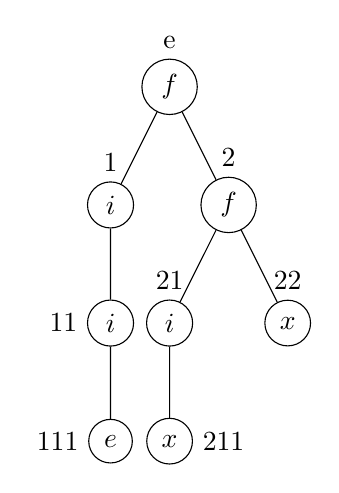
\begin{tikzpicture}
    \node [circle,draw][label=e]{$f$} child {node
      [circle,draw][label=1]{$i$}
      child{node[circle,draw][label=left:11]{$i$}
        child{node[circle,draw][label=left:111]{$e$}}}} child {node
      [circle,draw][label=2]{$f$} child {node
        [circle,draw][label=21]{$i$}
        child{node[circle,draw][label=right:211]{$x$}}} child {node
        [circle,draw][label=22]{$x$}} };
  \end{tikzpicture}
  \caption{Representación de $f(i(i(e)),f(i(x),x))$ en forma de
    árbol.}
\end{figure}

Las definiciones anteriores se pueden ver más claras con esta
representación. El conjunto de variables de un término $t$ son las
hojas del árbol, la longitud es el número de nodos del árbol, y el
tamaño es el numero de nodos del árbol menos sus hojas. Las variables
que se encuentren en las hojas de este árbol, las llamaremos variables
suelo.

En la figura \ref{fig:termino} cada nodo lleva una numeración. Esto
es lo que conocemos en términos como la posición. Nos resultará útil a
la hora de definir subtérminos y de dotar de cierta estructura al
concepto de término.

\begin{defi}
  Sea $\Sigma$ una signatura, $X$ un conjunto de variables disjuntas
  de $\Sigma$, y $s \in T(\Sigma, X)$. El conjunto posiciones
  $\Pos (s)$ se define de manera recursiva como,
\begin{itemize}

\item Si $s \in X$, entonces $\Pos(s) := {\epsilon}$, donde $\epsilon$
  es la cadena vacía.
\item Si $s = f(s_1, \dots, s_n)$ entonces,
$$ \Pos(s) := \{\epsilon\} \cup \{1p | p \in Pos(s_1) \} \cup \dots \cup \{np | p \in \Pos(s_n) \}$$
\end{itemize}
\end{defi}

El conjunto de $\Pos(s)$ serán cadenas de números naturales
positivos. Por ejemplo,
$\Pos f(f(i(i(e)),f(i(x),x))) = \{ \epsilon,1,11,111,2,21,211,22 \}$.

La implementaremos en Haskell bajo el nombre de la función \texttt{conjuntoPos t}\index{\texttt{conjuntoPos}}.

\begin{sesion}
>>> conjuntoPos (V ("x",1))
[[]]
>>> conjuntoPos (T "f" [V("x",1)])
[[],[1]]
>>> conjuntoPos (T "f" [T "i" [T "i" [T "e" []]],
                   T "f" [T "i" [V("x",1)], V("x",1)]])
[[],[1],[1,1],[1,1,1],[2],[2,1],[2,1,1],[2,2]]
\end{sesion}

Su definición es,

\begin{codigo}
conjuntoPos :: Termino -> [[Int]]
conjuntoPos (V _) = [[]]
conjuntoPos (T _ (xs)) = conjuntoPos' (reverse zs)
    where zs = (zip xs [1..])
          conjuntoPos' [] = [[]]
          conjuntoPos' ((t,n):ts) = (conjuntoPos' ts) ++ 
                                    (map (n:) (conjuntoPos t))
\end{codigo}


A continuación, introducimos la noción de subtérmino.
\begin{defi}
  Sea $s \in T(\Sigma, X)$ y $p \in \Pos (s)$. El subtérmino de $s$ en
  la posición $p$, denotado por $s|_p$ se define por inducción
  \begin{equation*}
    \begin{array}{rcl}
      s|_\epsilon & :=  & s \\
      f(s_1,\dots,s_n)|_{iq} & : = & s_i|_q \\
    \end{array}
  \end{equation*}
\end{defi}

De la misma manera, podemos extrapolar este concepto a los árboles. Un
término $t$ es subtérmino del término $s$, si el árbol generado por el
término $t$ es un subárbol para el árbol generado por $s$. 

Implementamos la función \texttt{esSubtermino t s} \index{\texttt{esSubtermino}}que comprueba si $t$ es
subtérmino de $s$. Por ejemplo,

\begin{sesion}
>>> esSubtermino (V ("x",1)) (T "f" [V("x",1)])
True
>>> esSubtermino (V ("x",2)) (T "f" [V("x",1)])
False
\end{sesion}

Queda implementada de la siguiente manera,

\begin{codigo}
esSubtermino :: Termino -> Termino -> Bool
esSubtermino t s@(T _ xs)
    | t == s = True
    | otherwise = or (map (esSubtermino t) xs)
esSubtermino t s = t == s
\end{codigo}

Una función que usaremos en los capítulos siguientes es
\texttt{ocurre v t}\index{\texttt{ocurre}}, que es la función \texttt{esSubtermino}
restringido a variables. A partir de ahora diremos que $v$ ocurre en
$t$ si la variable $v$ es subtérmino de $t$. Por ejemplo,

\begin{sesion}
>>> ocurre ("x",2) (V ("x",2)) 
True
>>> ocurre ("x",3) (V ("x",2)) 
False
>>> ocurre ("x",2) (T "f" [V ("x",2), T "g" [V ("x",2)]])
True
>>> ocurre ("y",5) (T "f" [V ("x",2), T "g" [V ("x",2)]])
False
\end{sesion}

Dado la naturaleza de la restricción variables, podríamos definir
\texttt{ocurre} como,

\begin{codigo}
ocurre :: Nvariable -> Termino -> Bool
ocurre v t = esSubtermino (V v) t
\end{codigo}

Sin embargo, podemos mejorar la definición sin usar la función
\texttt{esSubtermino},

\begin{codigo}
ocurre :: Nvariable -> Termino -> Bool
ocurre a (V x)    = a == x
ocurre a (T _ ts) = any (ocurre a) ts
\end{codigo}

Con la noción de subtérmino, introducimos una nueva función de
términos en términos. La idea es, a partir de $p\in \Pos(s)$ y de dos
términos $s,t$ sustituir el subtérmino $s|_p$ por $t$. En la
noción de árbol, sería cambiar todo el subárbol $s|_p$ por $t$,
dejando el resto de $s$ intacto. 

% INTRODUCIR UN DIBUJO


Formalmente lo definimos como sigue,

\begin{defi}
Sea $p \in Pos(s)$. Denotamos $s[t]_p$ como,
  \begin{equation*}
    \begin{array}{rcl}
      s[t]_\epsilon & :=  & t \\
      f(s_1,\dots,s_n)[t]|_{iq} & : = & f(s_1,\dots,s_i[t]_q,\dots,s_n) \\
    \end{array}
  \end{equation*}
\end{defi}

La función que calcule el término resultante la llamaremos
\texttt{sustPosSubtermino}\index{\texttt{sustPosSubtermino}}. Debemos tener en cuenta que la de
definición depende de la posición, por ello añadiremos una excepción
si $p$ no esta bien definido. Por ejemplo,

\begin{sesion}
>>> sustPosSubtermino (T "f" [V ("s",1),V ("s",2),V ("s",3)]) 
                        (V ("t",1)) [2,1]
T "f" [V ("s",1),V ("t",1),V ("s",3)]
sustPosSubtermino (T "f" [V ("s",1),V ("s",2),V ("s",3)]) 
                  (V ("t",1)) []
(V ("t",1))
sustPosSubtermino (V ("s",1)) (V ("t",1)) [2]
*** Exception: No se ha definido bien la lista de posiciones
>>> sustPosSubtermino (T "f" [V ("s",1),V("s",2),V("s",3)]) 
                        (V ("t",1)) [2,2]
T "f" [V ("s",1),*** Exception: No se ha definido bien la 
                     lista de posiciones
\end{sesion}

Su definición es,

\begin{codigo}
sustPosSubtermino :: Termino -> Termino -> [Int] -> Termino
sustPosSubtermino _ t [] = t
sustPosSubtermino (V _) t [1] = t
sustPosSubtermino (V _) _ _ = error("No se ha definido bien la 
                                     lista de posiciones")
sustPosSubtermino (T f xs) t (i:is) = (T f
    ((take (i-1) xs) ++
    (sustPosSubtermino (xs!!(i-1)) t is) :
    (drop i xs)))
\end{codigo}

\section {Sustituciones}

En esta sección vamos a introducir el concepto de sustituciones entre
términos. De manera general, una sustitución será una aplicación desde
un conjunto de las variables hacia el de los términos. Por ejemplo,
sea $f(x)$ un término $t$ y $\{x \mapsto i(x) \}$ la sustitución
$\tilde{\sigma}$. Si aplicamos $\tilde{\sigma}$ a $t$ obtenemos
$\tilde{\sigma}(t) = f(i(x))$. Formalmente la definiremos como sigue,

\begin{defi} 
  Sea $\Sigma$ una signatura y $X$ un conjunto infinito numerable de
  variables. Una $T(\Sigma, X)$--sustitución, es una función
  $\sigma : X \rightarrow T(\Sigma, X)$ tal que $\sigma(x) \neq x$
  para un número finito de variables $x \in X$. El conjunto de
  variables donde $\sigma(x) \neq x$ se le llama dominio de
  $\sigma$. Lo denotaremos por $\Dom (\sigma)$.
\end{defi}

En definitiva, las sustituciones son de la forma
$$\sigma = \{ x_1 \mapsto \sigma(x_1), \dots, x_n \mapsto \sigma(x_n)\}$$ 
entendiendo que las restantes variables se aplican en ellas mismas.

La implementación del tipo de dato
\texttt{Sustitucion}\index{\texttt{Sustitucion}} en Haskell es,

\begin{codigo}
  type Sustitucion = [(Nvariable,Termino)]
\end{codigo}

Por ejemplo, la sustitución
$\sigma = \{ x_2 \mapsto a, y_4 \mapsto z_5, v_1 \mapsto f(w_2) \}$ 
se representa por 
\begin{sesion}
[(("x",2),T "a" []),
 (("y",4),(V ("z",5))),
 (("v",1),T "f" [V ("w",2)])]
\end{sesion}

Para comprobar si una variable está en el dominio de una sustitución, definimos
la función \texttt{enDominio}\index{\texttt{enDominio}}, tal que \texttt{(enDominio x s)} se verifica si
\texttt{x} está en el dominio de \texttt{s}. Por ejemplo,

\begin{sesion}
>>> let s = [(("x",2),T "a" []),(("y",4),(V ("z",5)))]
>>> enDominio ("x",2) s
True
>>> enDominio ("x",3) s
False
>>> enDominio ("y",2) s
False
>>> enDominio ("y",4) s
True
>>> enDominio ("z",5) s
False
\end{sesion}

Su definición es:

\begin{codigo}
enDominio :: Nvariable -> Sustitucion -> Bool 
enDominio v = any (\(x,_) -> v == x)
\end{codigo}

Con la función \texttt{(aplicaVar s v)}\index{\texttt{aplicaVar}}, calculamos el término
obtenido tras aplicar una sustitución \texttt{s} a una variable
\texttt{v}. Por ejemplo,

\begin{sesion}
let s = [(("x",2),T "a" []),(("y",4),(V ("z",5)))]
>>> aplicaVar s ("x",2)
T "a" []
>>> aplicaVar s ("x",3)
V ("x",3)
>>> aplicaVar s ("y",2)
V ("y",2)
>>> aplicaVar s ("y",4)
V ("z",5)
>>> aplicaVar s ("z",5)
V ("z",5)
\end{sesion}

Su definición es:

\begin{codigo}
aplicaVar :: Sustitucion -> Nvariable -> Termino 
aplicaVar [] z = V z 
aplicaVar ((x,y):s) z 
  | x == z    = y
  | otherwise = aplicaVar s z
\end{codigo}

La definición de sustitución se puede extender para términos
$t \in T(\Sigma, X)$. Sea la extensión $\tilde{\sigma}$ definida como,

\begin{equation*}
  \tilde{\sigma}(t)=
  \left\lbrace
    \begin{array}{ll}
      \tilde{\sigma}(x) = \sigma(x) 
        & \text{si } t \in X \\
      \tilde{\sigma}(f(t_1, \dots, t_n)) = f(\tilde{\sigma}(t_1), \dots, \tilde{\sigma}(t_n)) 
        & \text{si } t = f(t_1, \dots, t_n)
    \end{array}
  \right.
\end{equation*}

A partir de ahora, entenderemos $\sigma$ como una sustitución
extendida, a menos que se indique lo contrario.

Para la computación de esta definición usamos la función
\texttt{(aplicaTerm s t)}\index{\texttt{aplicaTerm}}, que es el término obtenido tras aplicar la
sustitución \texttt{s} al término \texttt{t}. Por ejemplo,

\begin{sesion}
>>> let s = [(("x",2),T "a" []),(("y",4),(V ("z",5)))]
>>> aplicaTerm s (T "s" [V ("x",2), T "m" [V ("y",4)]])
T "s" [T "a" [],T "m" [V ("z",5)]]
>>> aplicaTerm s (T "s" [V ("x",4), T "m" [V ("y",2)]])
T "s" [V ("x",4),T "m" [V ("y",2)]]
\end{sesion}

Su definición es:

\begin{codigo}
aplicaTerm :: Sustitucion -> Termino -> Termino
aplicaTerm s (V x)    = aplicaVar s x
aplicaTerm s (T f ts) = T f (map (aplicaTerm s) ts)
\end{codigo}

Como la sustituciones son muy parecidas a las funciones, podemos
plantearnos la composición entre ellas. Definiéndolas como $\sigma\tau(x) :=
\tilde{\sigma}(\tau(x))$. Veamos que $\sigma\tau(x)$ es una sustitución

\begin{lema}
  La composición de sustituciones es una sustitución.
\end{lema}

\begin{demo}
  $\sigma\tau(x)$ es una función de $X$ a $T(\Sigma, X)$. Como
  $\sigma\tau(x) = x$ ocurre para todas las variables
  $x\in V - (\Dom(\sigma)\cup \Dom(\tau))$, por definición, es una
  sustitución.
\end{demo}

A continuación, introducimos un nuevo concepto imprescindible para la reescritura.

\begin{defi}
  Sea $\Sigma$ una signatura y $X$ un conjunto finito numerable de variables
  disjuntas de $\sigma$. Una identidad es un par
  $(s,t) \in T(\Sigma, X) \times T(\Sigma, X)$. Las denotaremos por
  $s \approx t$, donde $s$ lo denominaremos el lado izquierdo y $t$ el lado
  derecho.
\end{defi} 

La idea de esta definición es similar a lo que entendemos por
equivalencia. Por ejemplo, en la definición de grupos tenemos la
propiedad asociativa, $(a+b)+c =a+(b+c)$. De la misma manera podemos
representar la propiedad como una identidad de $\Sigma_G$,
$f(f(a,b),c) \approx f(a,f(b,c))$.

Podemos relacionar este concepto con lo que hemos visto en el capítulo 1.

\begin{defi}
  Sea $E$ un conjunto de identidades de $\Sigma$. La relación de
  reducción $\rightarrow_E \subseteq T(\Sigma, V) \times T(\Sigma, V)$
  se define como,
  \[
    s \rightarrow_E t \hspace{.3cm} syss \hspace{.3cm} \exists(l,r)
    \in E, p \in \Pos (s), \sigma \text{ una sustitución tal que } s|_p = \sigma(l) \text{ y } t=
    s[\sigma(r)]_p.
  \]
\end{defi}

Volviendo al ejemplo de grupos, su conjunto de identidades es,
\[
  G : = \{f(x,f(y,z)) \approx f(f(x,y),z), f(e,x) \approx x, f(i(x),x)
  \approx e \}
\]
El término $f(i(a), f(a,e))$, con $a$ una constante, tiene una
reducción en la posición $\epsilon$ con la sustitución
$\sigma = \{x \mapsto i(a), y \mapsto a, z \mapsto e \}$, y es
$f(f(i(a),a),e)$. Podemos afirmar nuevamente que
$f(f(i(a),a),e) \rightarrow_G f(e,e)$, en la posición $1$ y la
sustitución $\sigma = \{x \mapsto a \}$.

% Añadir un dibujo


\section{Caracterización de $\xleftrightarrow{*}_E$}

Como hemos visto en el capítulo 1, la clausura transitiva reflexiva de
$\rightarrow_E$ la denotamos por $\xrightarrow{*}_E$, y la clausura
simétrica transitiva reflexiva por $\xleftrightarrow{*}_E$. En la
última parte de este capítulo, vamos a dar una caracterización de
$\xleftrightarrow{*}_E$ que usaremos en capítulos posteriores.

\begin{defi} 
  Sea $\equiv$ una relación binaria en $T(\Sigma,V)$
  \begin{enumerate}
  \item La relación $\equiv$ es cerrada bajo sustituciones syss $s \equiv t$
    implica $\sigma(s) \equiv \sigma(t)$, para todo $s,t$ y $\sigma$. 
  \item La relación $\equiv$ es cerrada bajo $\Sigma$--operaciones syss $s_1
    \equiv t_1, \dots, s_n \equiv t_n$ implica $f(s_1, \dots, s_n) \equiv
    f(t_1, \dots, t_n)$, para todo $n \geq 0, f, s_1, \dots s_n, t_1, \dots
    t_n.$ 
  \item La relación $\equiv$ es compatible con $\Sigma$--operaciones syss $ s
    \equiv t$ implica $f(s_1, \dots, s_{i-1},s, s_{i+1},\dots, s_n) \equiv
    f(s_1, \dots, s_{i-1},t, s_{i+1},\dots, s_n)$ para todo $n \geq 0, f, i =
    1, \dots, n,$ y $s_1, \dots, s_{i-1},s,t, s_{i+1},\dots, s_n$. 
  \item La relación $\equiv$ es compatible con el $\Sigma$--contexto syss $s
    \equiv s'$ implica $t[s]_p \equiv t[s']_p$ para todo $t$ y $p$. 
  \end{enumerate}       
\end{defi}

Una consecuencia directa a partir de la definición de $\rightarrow_E$ es,

\begin{lema} \label{lema:2.1}
  Sea $E$ un conjunto de $\Sigma$--identidades. La relación de reducción de
  $\rightarrow_E$ es cerrada bajo sustitución y compatible con las
  $\Sigma$--operaciones.
\end{lema}

\begin{demo}
  Es trivial pues si sabemos que $s_i \equiv t_i \forall i$, entonces
  $\sigma(s_i) \equiv \sigma(t_i) \forall i$, y
  $f(s_1, \dots, s_n) \equiv f(t_1, \dots, t_n)$ por la propia
  definición de relación de reducción.
\end{demo}

Otro lema importante para la caracterización es,

\begin{lema} \label{lema:2.2}
  Sea $\equiv$ una relación binaria en $T(\Sigma,V)$.
  \begin{enumerate}
  \item La relación $\equiv$ es compatible con las
    $\Sigma$--operaciones syss es compatible con el
    $\Sigma$--contexto.
  \item Si $\equiv$ es reflexiva y transitiva, entonces es compatible
    con las $\Sigma$--operaciones syss es cerrado bajo las
    $\Sigma$--operaciones.
  \end{enumerate}
\end{lema}

\begin{demo}
  La primera propiedad de derecha a izquierda es trivial por la
  definición de posición. De izquierda a derecha se realiza mediante
  una inducción de $p$, como para $p= \epsilon$ la afirmación es
  cierta, también lo será para $p=p_1$, por tanto también para
  $p=p_1 p_2 \dots$.  La segunda propiedad de izquierda a derecha es
  cierta por la transitividad de $\equiv$. De derecha a izquierda se
  usa que la relación es reflexiva.
\end{demo}

\begin{teor} \label{teor:2.1}
  Sea $E$ un conjunto de $\Sigma$--identidades. La relación
  $\xleftrightarrow{*}_E$ es la relación de equivalencia más pequeña en
  $T(\Sigma,V)$ que contiene $E$ que es cerrada bajo sustituciones y
  $\Sigma$-operaciones.
\end{teor}

\begin{demo}
  $\xleftrightarrow{*}_E$ es una relación de equivalencia reflexiva y
  transitiva. Con el lema \ref{lema:2.1} tras aplicar inducción, se puede
  ver que es cerrada bajo sustituciones y compatible con
  $\Sigma$--operaciones. Por el lema \ref{lema:2.2}, también es cerrada bajo
  $\Sigma$--operaciones.

  Vamos a suponer que existe $\equiv$ relación de equivalencia en
  $T(\Sigma,v)$ que contiene a $E$, y es cerrada bajo sustituciones y
  $\Sigma$--operaciones. Nuestro objetivo es comprobar que
  $\xleftrightarrow{*} \subseteq \equiv$, para ello, demostraremos que
  si $s \rightarrow_E t$ entonces $s \equiv t$.

  Partiendo de $s \rightarrow_E$, por la definición de relación de
  reducción, existe $(l,r) \in E$, $p$ posición de $s$, y $\sigma$ una
  sustitución tal que $s|_p = \sigma(l)$ y $t= s [\sigma(r)]_p$. 

  Como $\equiv$ contiene a $E$ entonces $l \equiv r$, por tanto,
  $\sigma(l) \equiv \sigma(r)$ por ser cerrada bajo sustituciones.  Al
  ser $\equiv$ reflexiva y cerrada bajo $\Sigma$--operaciones y
  compatible con $\Sigma$--operaciones, por el lema \ref{lema:2.2} también
  es compatible con $\Sigma$--contexto y por la definición de la
  propiedad, $s = s[\sigma(l)]|_p \equiv s[\sigma(r)]|_p = t$.
\end{demo}

La demostración del teorema \ref{teor:2.1}, nos indica una manera de
calcular $\xleftrightarrow{*}_E$ a partir de $E$ mediante las
relaciones de reflexividad, simetría, transitividad, sustituciones,
y $\Sigma$--operaciones. La aplicación de estas reglas en este
contexto, es lo que llamamos lógica ecuacional. Las reglas se pueden escribir así,

\[
  \begin{array}{lc}
    $Reflexiva$     & \dfrac{}{E \vdash t \approx t} \\ \\
    $Sim\'{e}trica$         & \dfrac{E \vdash s \approx t}{E \vdash t \approx s} \\ \\
    $Transitiva$    & \dfrac{E \vdash s \approx t  \hspace{.8cm}   E \vdash t \approx u}{E \vdash s \approx u} \\ \\
    $Sustitución$   & \dfrac{E \vdash s\approx t}{E \vdash \sigma(s)\approx \sigma(t)} \\ \\
    \Sigma$--operaciones$    & \dfrac{E \vdash s_1\approx t_1 \hspace{.8cm} \dots \hspace{.8cm} E \vdash s_n\approx t_n}{E \vdash f(s_1, \dots, s_n) \approx f(t_1,\dots,t_n)}
  \end{array} 
\]


%%% Local Variables:
%%% mode: latex
%%% TeX-master: "SRT_en_Haskell"
%%% End:
